% ------------------------- MAIN TASK ---------------------------------
\section{Développement schématique}

\subsection{Choix des composants} \label{ssec:num32}
{
	\subsubsection{Microcontrôleur}
	Lors de la recherche de composants, j'ai décidé d'utiliser l'un des PIC32 standards de l'ES :
	\textbf{PIC32MX130F064D-I/PT}.
		
	\begin{figure}[h]
		\centering
		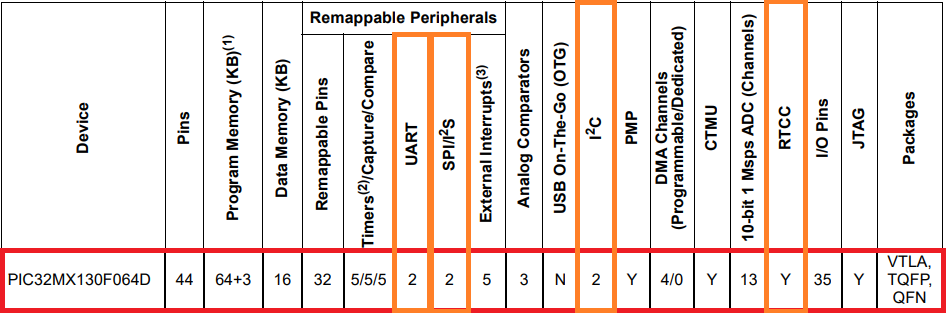
\includegraphics[width=1\linewidth]{Figures/Dev-SCH/PIC32-choisi}
		\caption{Périphériques disponibles du PIC}
		\label{fig:pic32-choisi}
		\source{PIC32MM0256GPM064 family datasheet}
	\end{figure}
	
	Nous pouvons constater sur la figure \ref{fig:pic32-choisi} que les critères minimaux de mon projet sont respectés :
	
	\begin{center}
		\fbox{\textit{1 - I2C}} \fbox{\textit{1 - SPI}} \fbox{\textit{1 - UART}} \fbox{\textit{1 - RTCC}}
	\end{center}
}

\clearpage
\subsection{Dimensionnements} \label{ssec:num31}
{
	\subsubsection{Vue d'ensemble schématique} \label{sssec:SchemaBloc} \vspace{-6mm}
	{
		\begin{figure}[th]
			\centering
			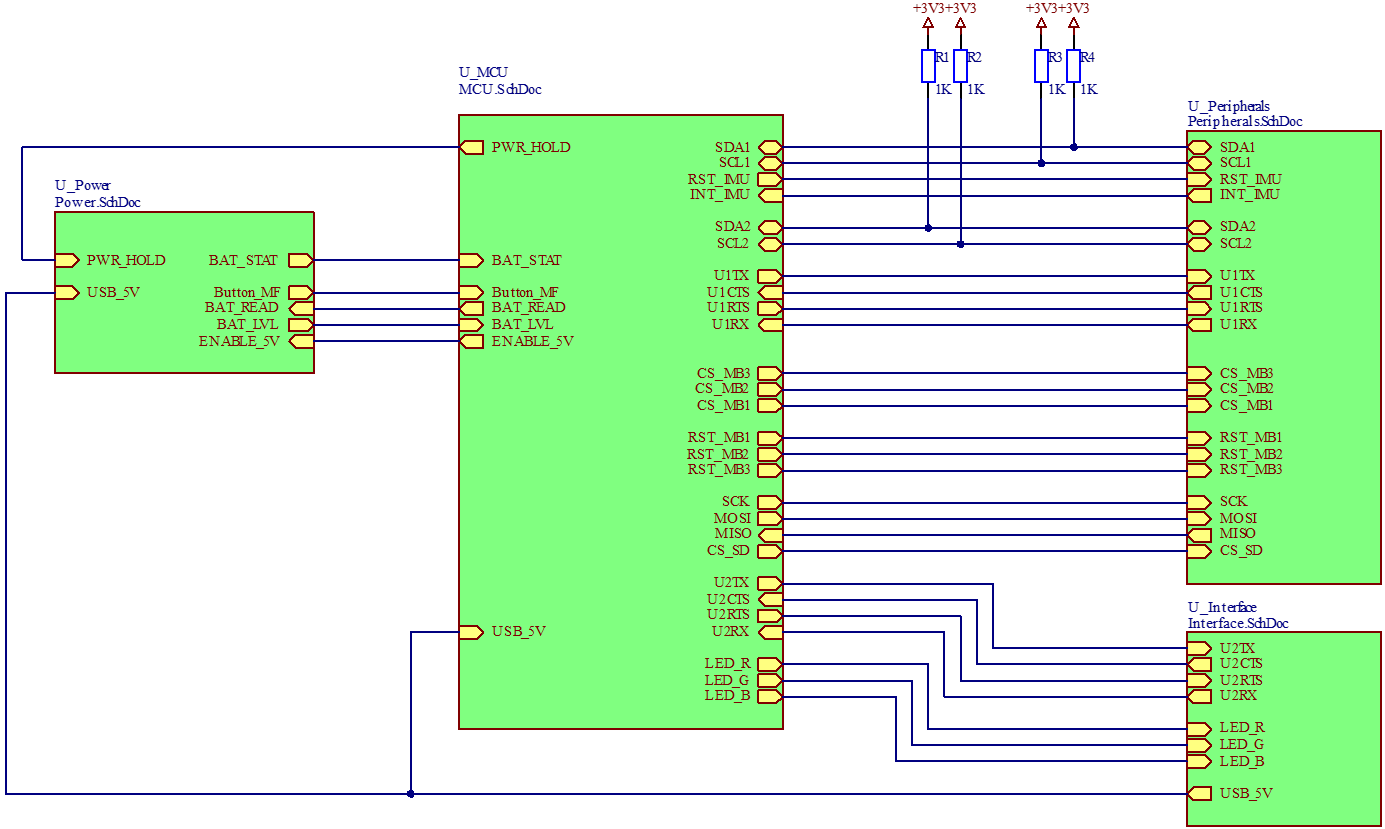
\includegraphics[width=1.1\linewidth]{Figures/Dev-SCH/schemaBloc}
			\caption{Schéma bloc de la schématique}
			\source{Auteur}
			\label{fig:schemablocSCH}
		\end{figure} \vspace{-5mm}
		Nous pouvons constater sur la figure \ref{fig:schemablocSCH} la structure des différents blocs du schéma : 
		
		\begin{tabularx}{18cm}{|X|X|}
			\hline
			Bloc & Description \\
			\hline
			\hline
			Power & Contient les différents régulateurs du système, ainsi que la gestion de charge de la batterie. \\
			\hline
			MCU & Contient l'intelligence du système, avec le microcontrôleur ainsi que tous ses composants passifs associés. \\
			\hline
			Peripherals & Périphériques du système : Carte-SD, Centrale inertielle, Capteur de pression, Slots MikroE. \\ 
			\hline
			Interface & Connecteur USB avec convertisseur serial (FTDI) et tous les composants passifs de sécurité. Interface LED RGB pour le statut. \\
			\hline
		\end{tabularx}
	}


	\clearpage
	\subsubsection{Autonomie du système} \label{sssec:SysAutonomie}
	{
		Afin de proportionner la batterie du circuit, il a fallut dimensionner les différentes consommations des composants, ceci par le biais de leurs documentations :
		
		\begin{center}
			\fbox{\textit{MCU - 30mA}} \fbox{\textit{BNO055 - 12.3mA}} \fbox{\textit{Capt. Pression - 4mA}} \fbox{\textit{\textcolor{red}{Carte-SD - 100mA}}} \fbox{\textit{MikroE - ??mA}} \fbox{\textit{Régulateurs - 40uA}} \fbox{\textit{LED RGB - 25mA}} 
		\end{center}
		
		Nous pouvons constater que la plus grande consommation vient de la carte micro-SD, qui au maximum peut induire 100mA. \footnote{Selon datasheet SanDisk : https://images-na.ssl-images-amazon.com/images/I/91tTtUMDM3L.pdf}
		
		
		Afin d'obtenir une autonomie d'au moins 2h (selon CDC), il faudrait une capacité de :
		
		\begin{equation}
			Capacite = Consommation_{tot} * Temps
		\end{equation}
		
		Ce qui nous fait une capacité de $\sim$342.68mAh, valeur facilement atteignable par les batteries li-ion du marché. Étant-donné que différents projets utilisaient des batteries 3400mAh, dans un objectif de conformité et de simplification des commandes, j'ai choisis cette même valeur.
		Ce qui signifie une autonomie de $\sim$20 heures, sans compter les différents mécanismes d'économie d'énergie.
		
		C'est un temps largement suffisant pour la durée de plusieurs expéditions, néanmoins la RTCC du microcontrôleur requiert d'être alimentée en permanence, j'ai donc décidé de déterminer un fonctionnement, où lorsque l'on charge la batterie la date se mettrait à jour et le mode "éteint" serait juste un mode de veille qui attendrait un niveau positif sur le switch avant de commencer le logging avec un timsetamp principale contenant la date, puis, seulement des deltas entre les mesures. Un diagramme des états est présents à la figure \ref{fig:etatsdiagramme}.
		
		\clearpage
		\begin{figure}[th]
			\centering
			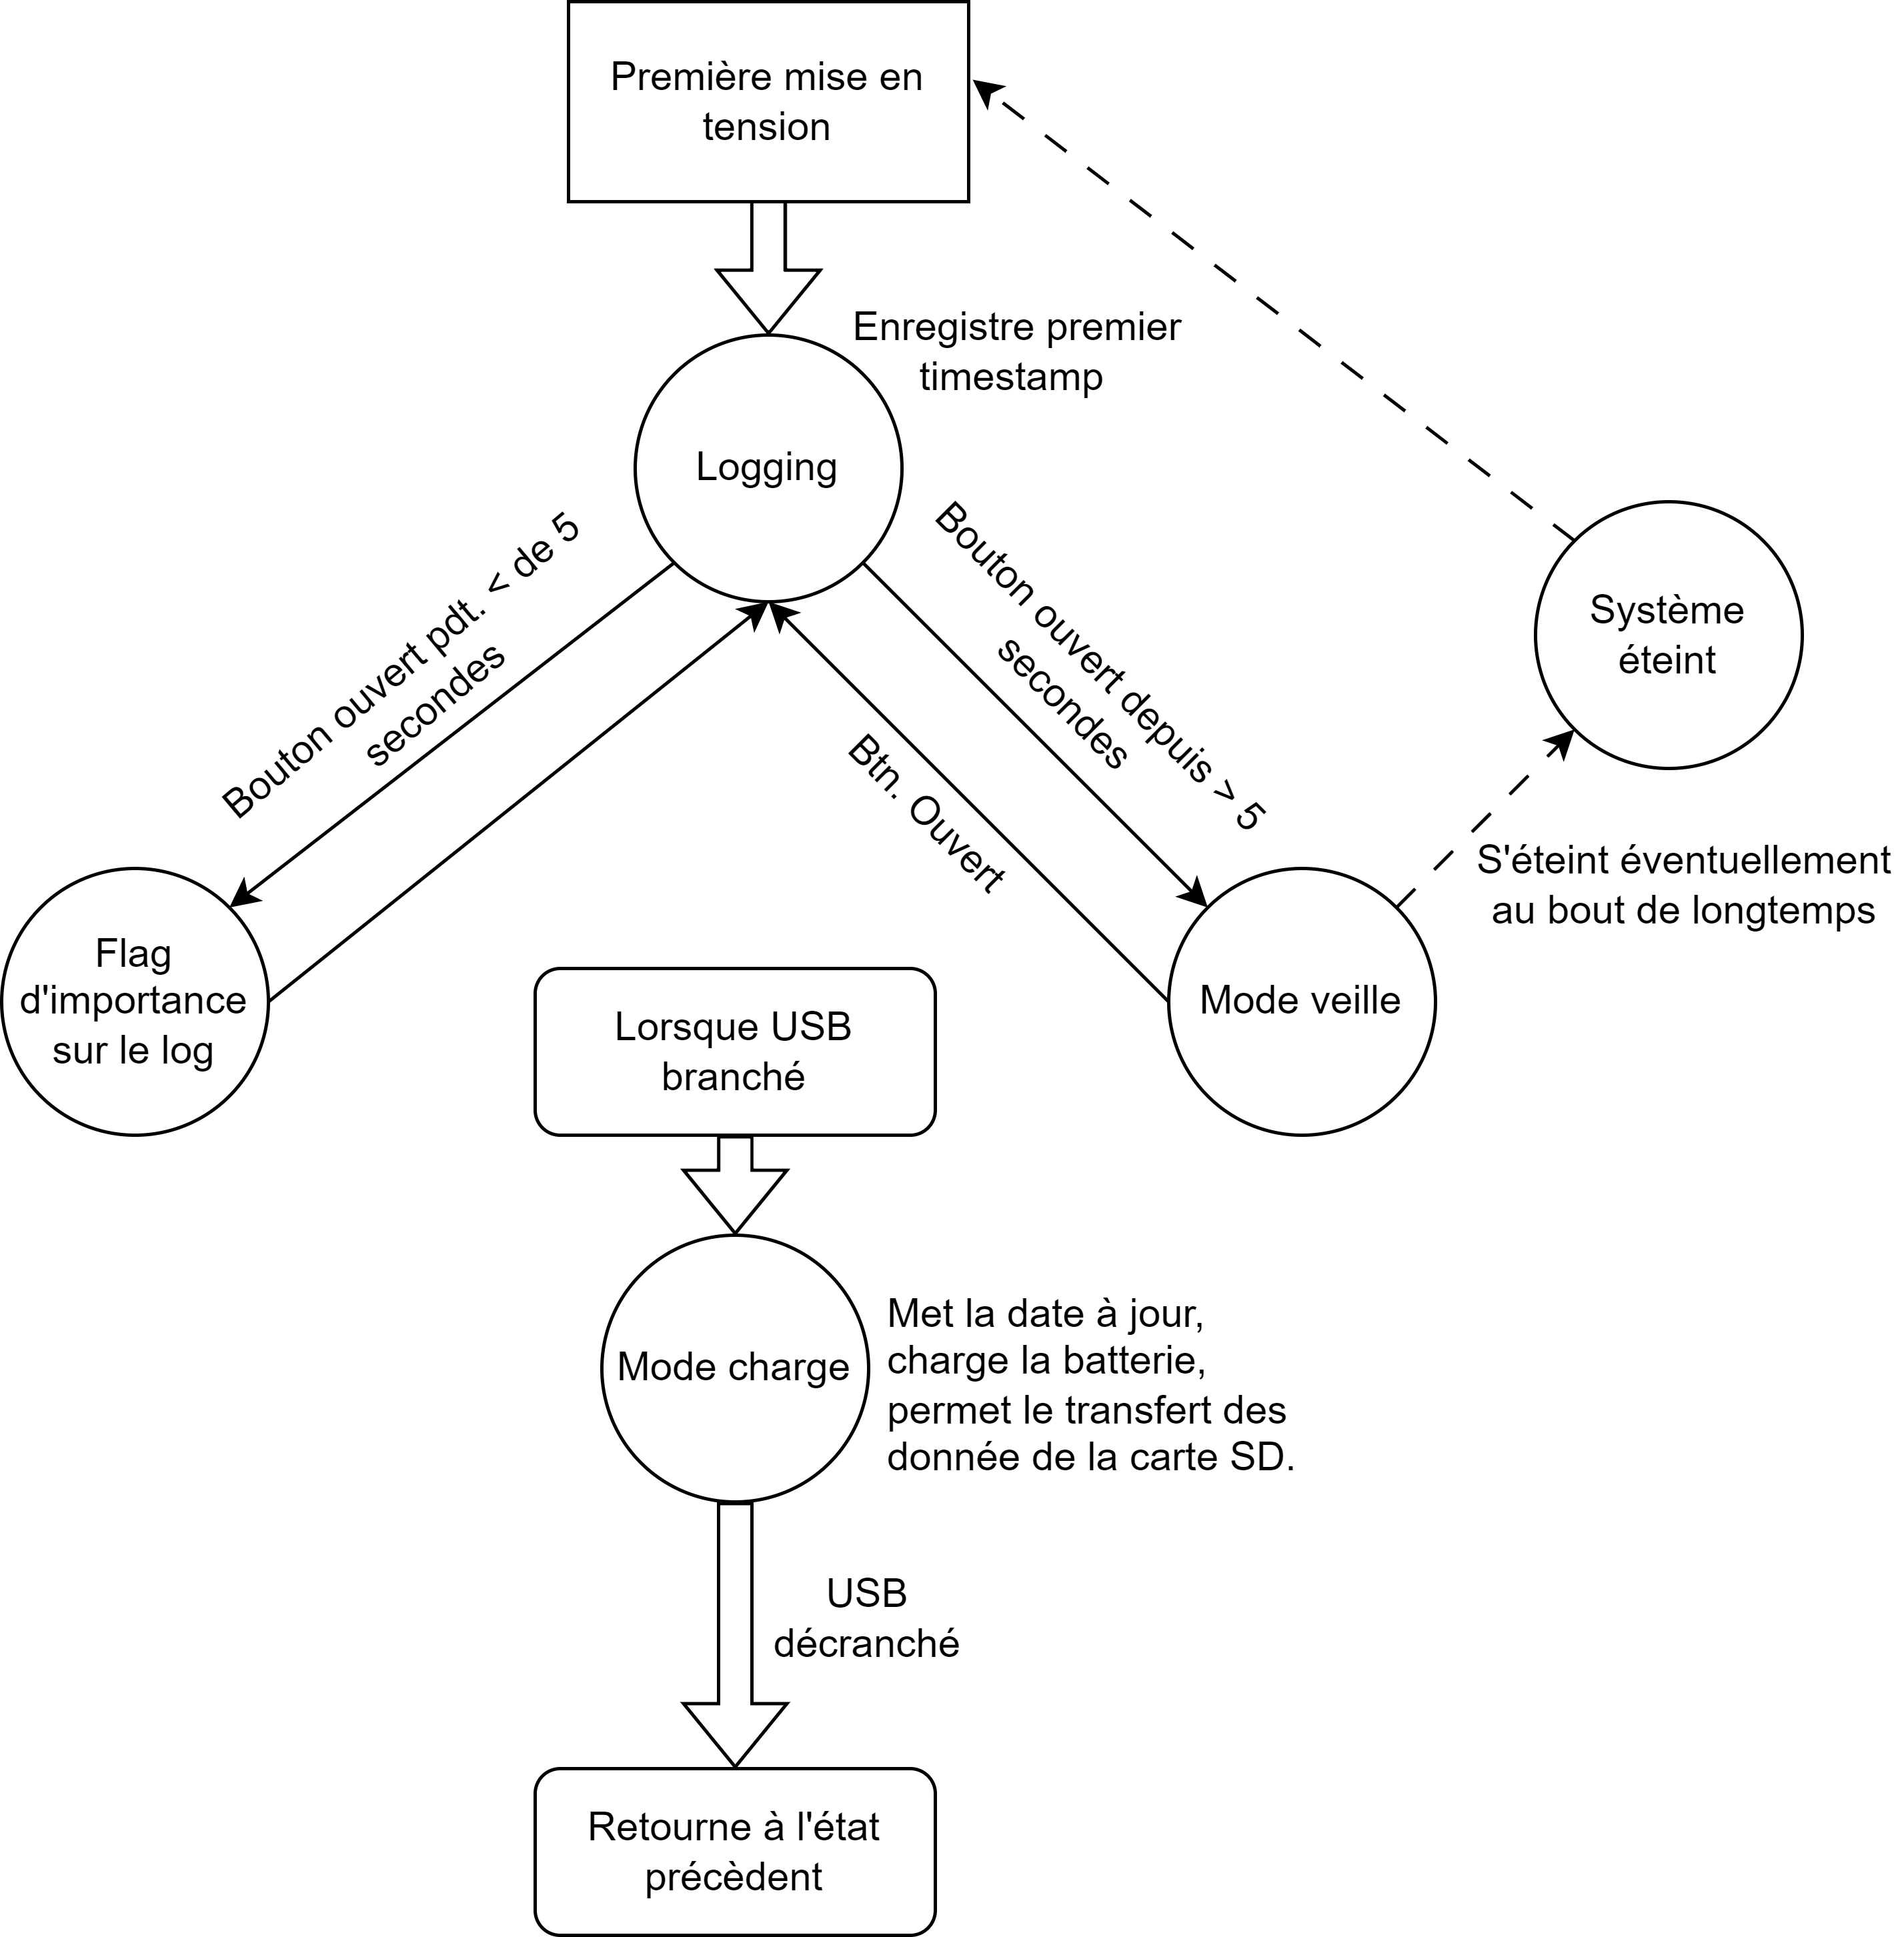
\includegraphics[width=1.1\linewidth]{Figures/Dev-SCH/Etats_diagramme}
			\caption{Diagramme des états du système}
			\label{fig:etatsdiagramme}
			\source{Auteur}
		\end{figure}
		
	}

	\clearpage
	\subsubsection{LED Interface} \label{sssec:DimLedRGB}
	{
		Afin d'informer l'utilisateur de ce qu'il se passe dans le système, j'ai décidé d'implémenter en tant qu'interface, une led RGB. Celle-ci sera un minimum puissante, afin de pouvoir être lisible lors de l'utilisation sous-marine du module.
		
		La consommation de la led RGB étant relativement importante, des mécanismes d'économie d'énergie seront mis en place dans le développement firmware. \vspace{+3mm}
		
		\textbf{Diagramme d'interface :}
		
		\begin{figure}[h]
			\centering
			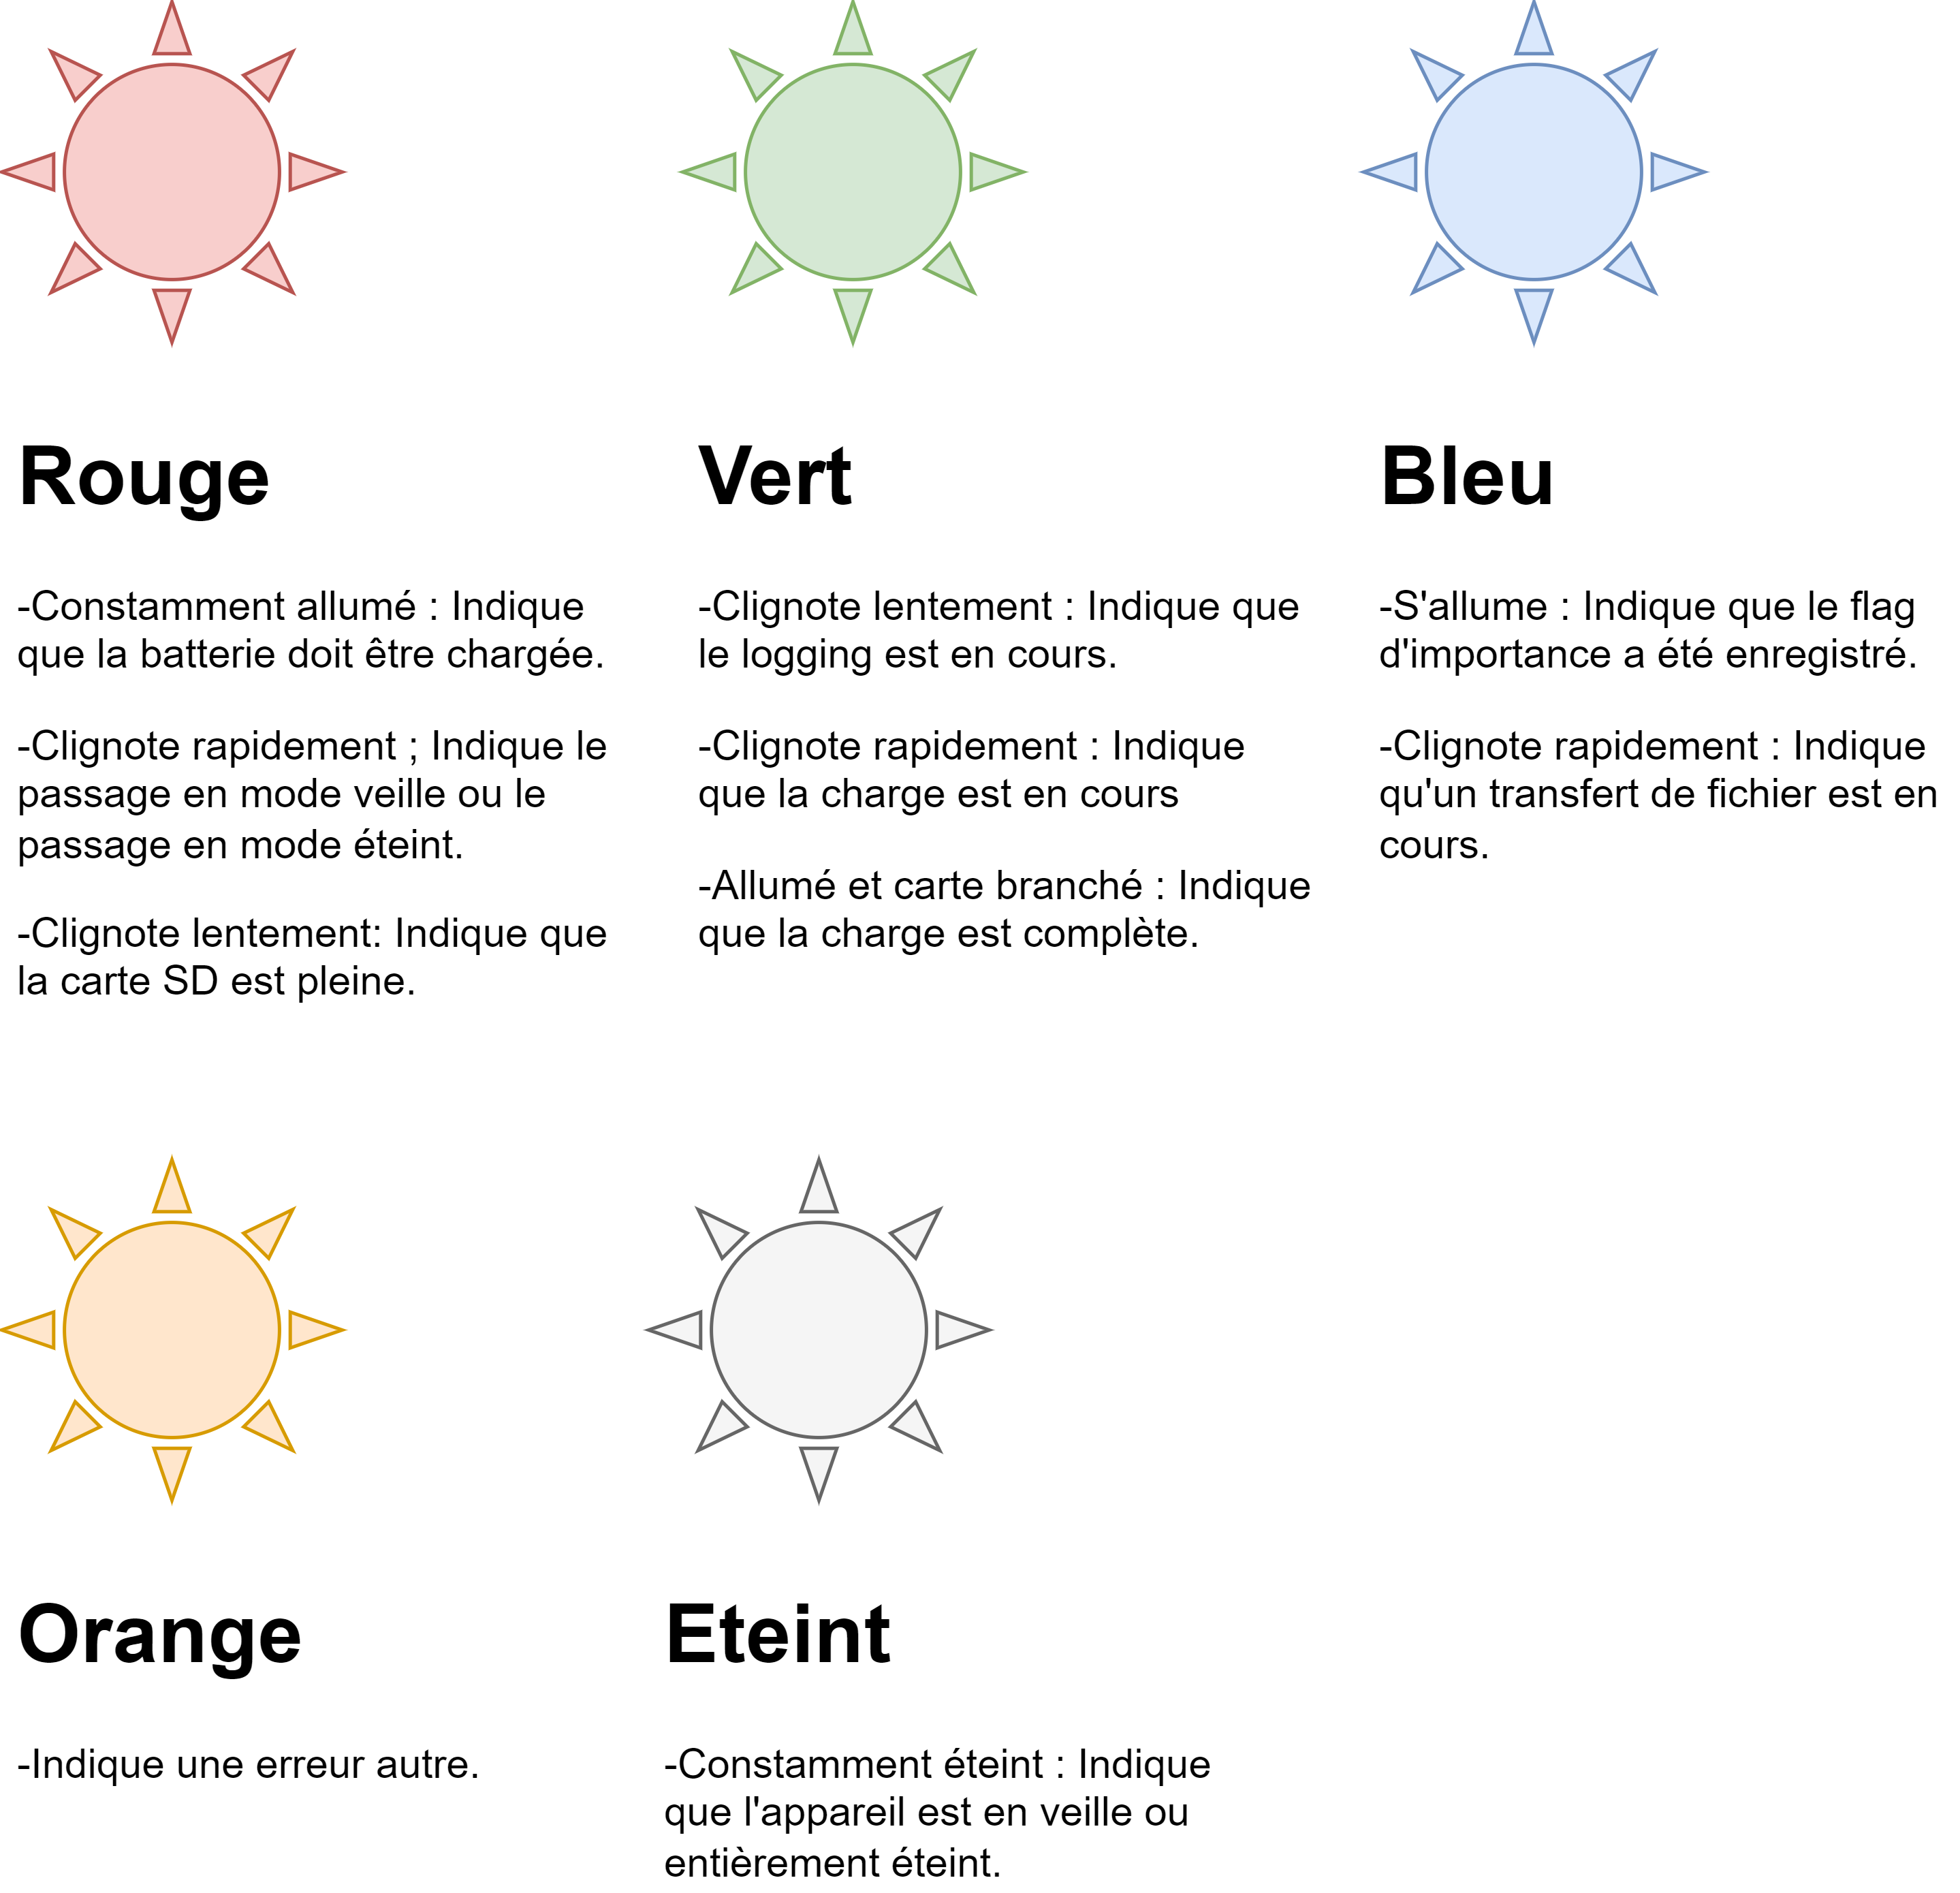
\includegraphics[width=0.95\linewidth]{Figures/Dev-SCH/LEDStates}
			\caption{Définitions des états de la LED RGB}
			\source{Auteur}
			\label{fig:ledstates}
		\end{figure}
	}

	\clearpage
	\subsubsection{Adaptation mécanique} \label{sssec:MecAdapt}
	{	
		L'idée étant d'obtenir une mesure de pression sans modification mécaniques sur le boîtier originale, plusieurs idées ont émergées :
		\begin{itemize}
			\item[1)] Mesurer une déformation mécanique a-même le module, dans le but de déduire la pression (Développement d'un capteur).
			\item[2)] Ajout d'une rallonge cylindrique au module, afin de fixer un capteur de pression à plat sur celui-ci, tout en permettant les modifications mécaniques sans altération du boîtier originale.
		\end{itemize}
		Par sa complexité moins importante et due aux contraintes de temps, la seconde option sera-celle développée lors de cette version du projet.
		Voici des ébauches (Pas à l'échelle) du concept : 
		\begin{figure}[h]
			\centering
			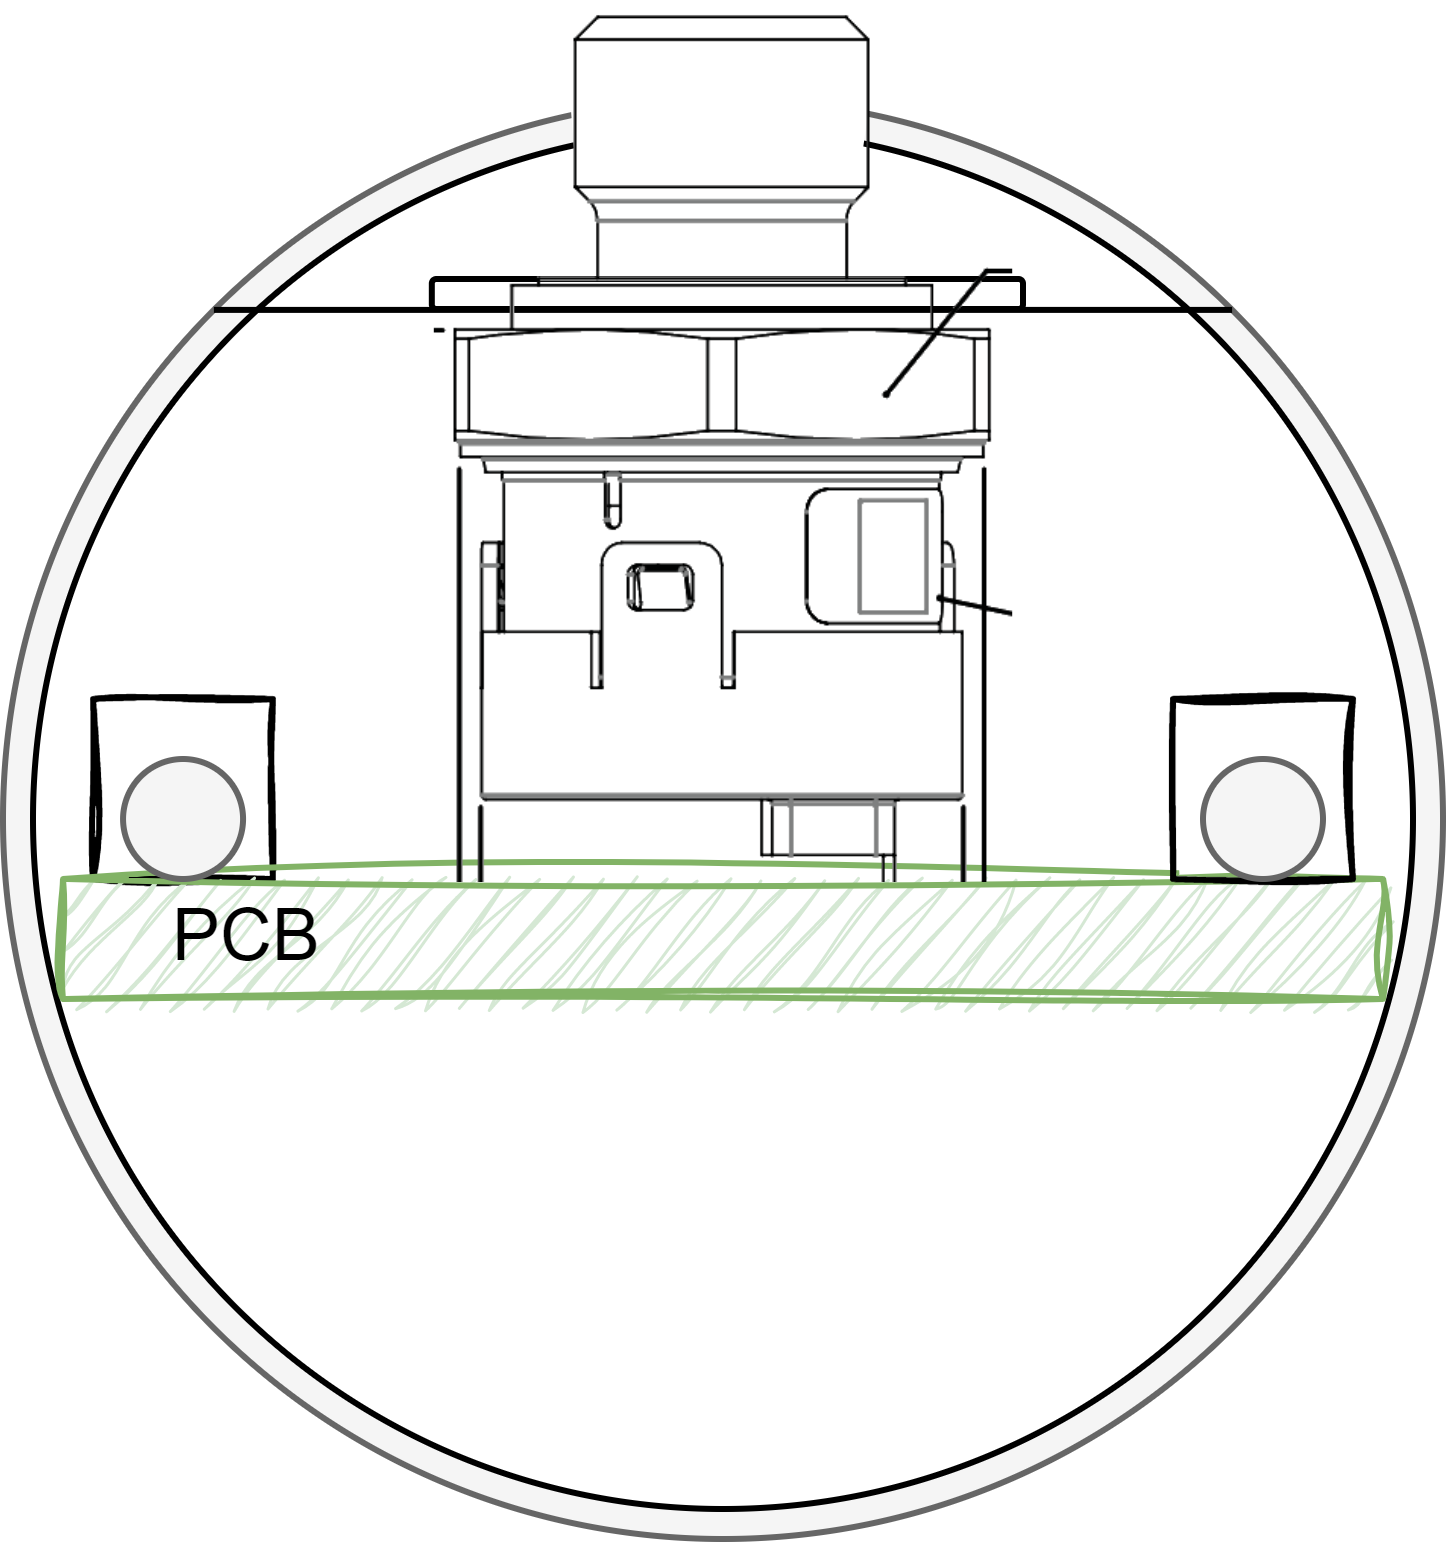
\includegraphics[width=0.45\linewidth]{Figures/Dev-SCH/MecaniqueProto1}
			\caption{Ébauche intérieur du cylindre}
			\label{fig:mecaniqueproto1}
			\source{Auteur}
		\end{figure}\vspace{-5mm}
		\begin{figure}[!h]
			\centering
			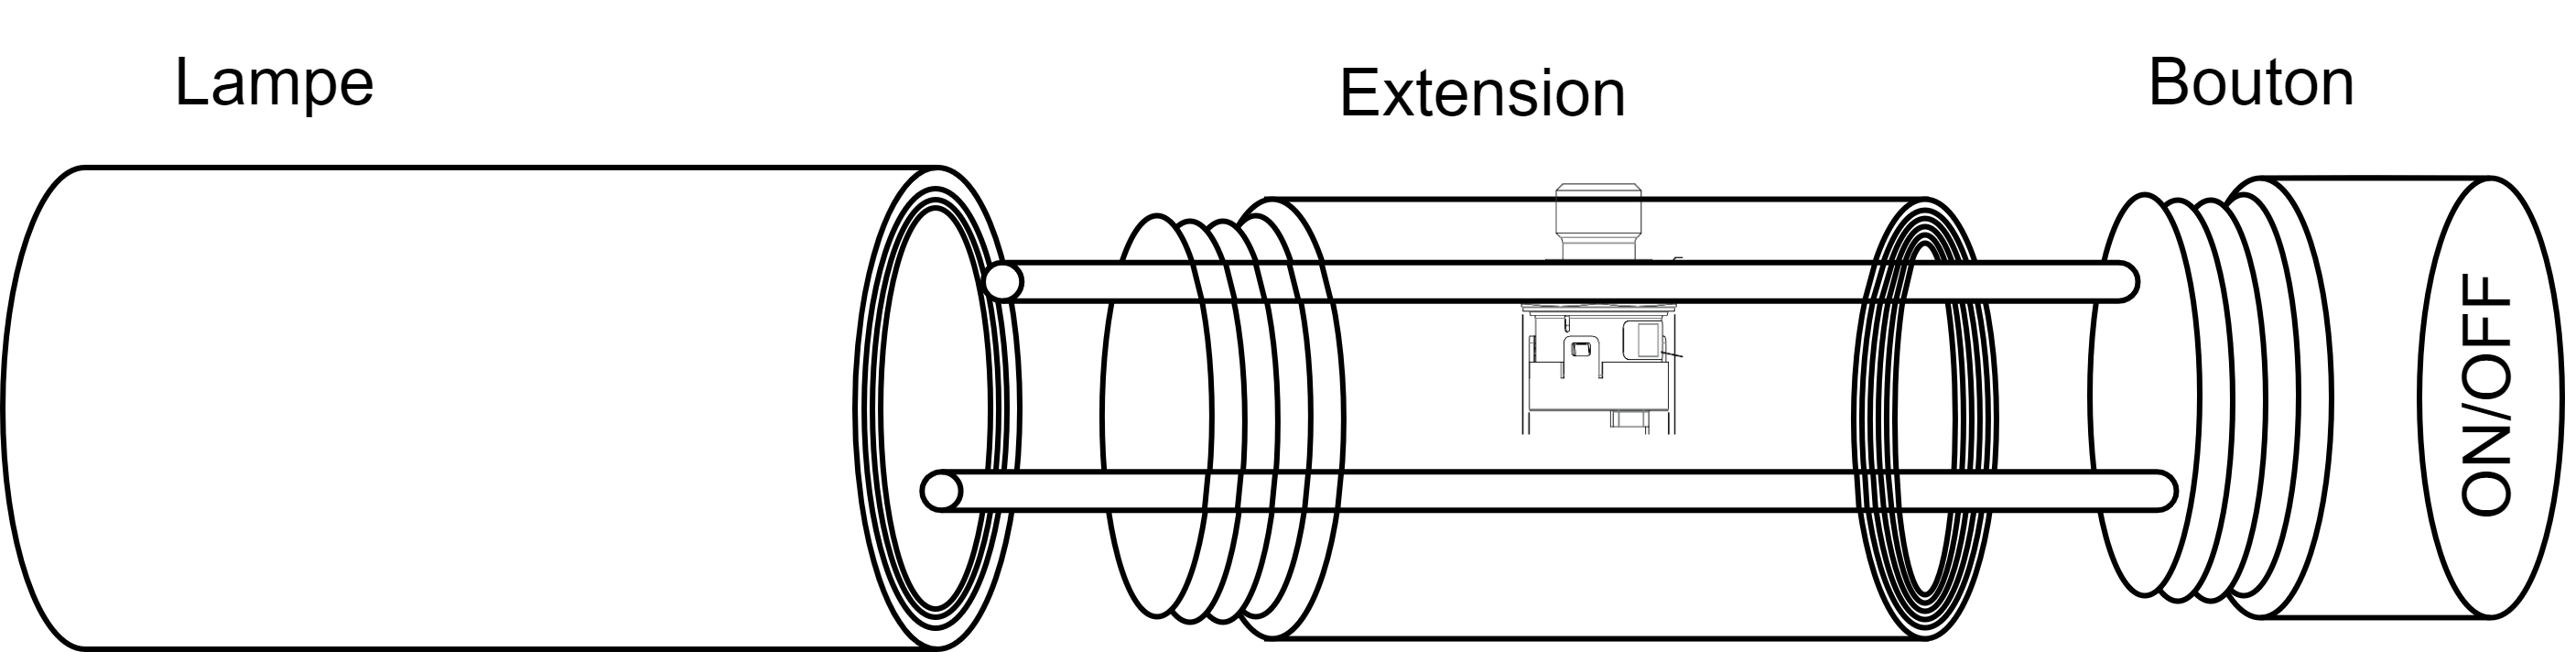
\includegraphics[width=0.75\linewidth]{Figures/Dev-SCH/MecaniqueProto2}
			\caption{Ébauche globale}
			\label{fig:mecaniqueproto2}
			\source{Auteur}
		\end{figure}
		
		
	}

	\clearpage
	\subsubsection{Bus de communications}
	{
		\textbf{UART (1) :} \\
		\underline{Utilisation :} Communication avec les boards Mikroe, pour les clicks-boards utilisant la comm. série. \\
		\underline{Pinning :} \vspace{-6mm}
		\begin{figure}[h]
			\centering
			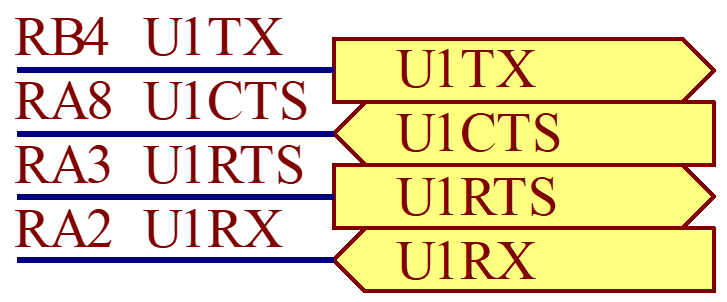
\includegraphics[width=0.25\linewidth]{Figures/Dev-SCH/UART1}
			\label{fig:uart1}
		\end{figure}		
	
		\textbf{UART (2) :} \\
		\underline{Utilisation :} Communication avec FTDI conversion USB-Serial. Transfert des fichiers de la carte-SD et mise-à-jour de la RTCC. \\
		\underline{Pinning :} \vspace{-6mm}
		\begin{figure}[h]
			\centering
			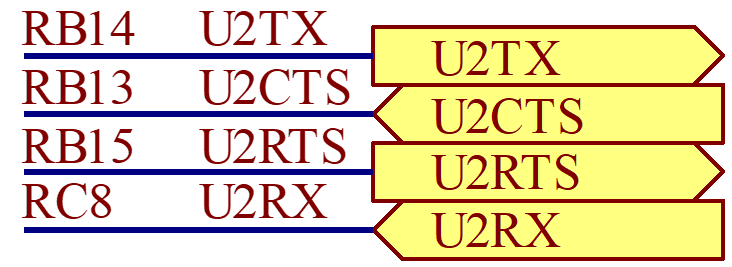
\includegraphics[width=0.25\linewidth]{Figures/Dev-SCH/UART2}
			\label{fig:uart2}
		\end{figure}		
	
		\textbf{SPI :} \\
		\underline{Utilisation :} Communication avec la carte micro-SD, écriture des mesures, timestamps et flag d'importance. \\
		\underline{Pinning :} \vspace{-6mm}
		\begin{figure}[h]
			\centering
			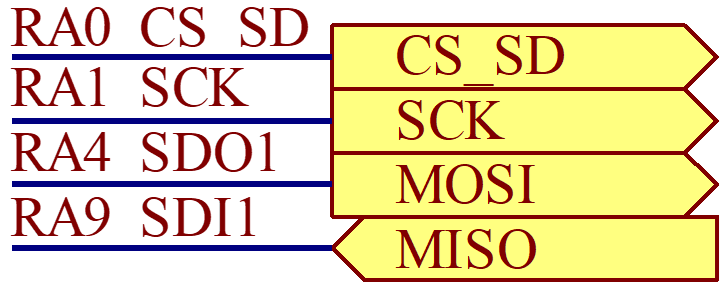
\includegraphics[width=0.25\linewidth]{Figures/Dev-SCH/SPI}
			\label{fig:spi}
		\end{figure}
	
		\textbf{I2C (1) :} \\
		\underline{Utilisation :} Lecture des mesure de la centrale inertielle BNO055 et paramétrage des registres de celui-ci. \\
		\underline{Pinning :} \vspace{-6mm}
		\begin{figure}[h!]
			\centering
			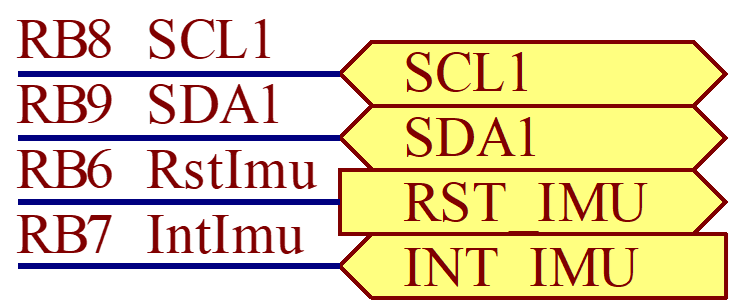
\includegraphics[width=0.25\linewidth]{Figures/Dev-SCH/I2C1}
			\label{fig:i2c1}
		\end{figure}
	
		\textbf{I2C (2) :} \\
		\underline{Utilisation :} Lecture des données du capteur de pression et est également connecté aux slots Mikroe, pour permettre à ceux-ci de communiquer via I2C. \\
		\underline{Pinning :} \vspace{-6mm}
		\begin{figure}[h!]
			\centering
			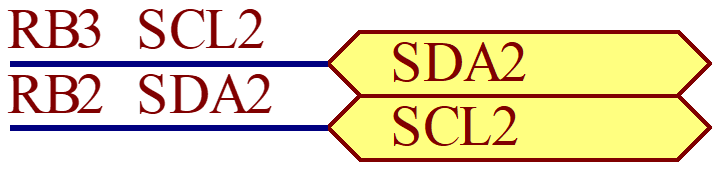
\includegraphics[width=0.25\linewidth]{Figures/Dev-SCH/I2C2}
			\label{fig:i2c2}
		\end{figure}
	
		\clearpage
		Pour ce qui est des mesures sur ces différents bus de communications, des connecteurs bergs ont étés prévus, afin de pouvoir connecter facilement un analyseur logique sur les différentes trames : 
		
		\begin{figure}[h]
			\centering
			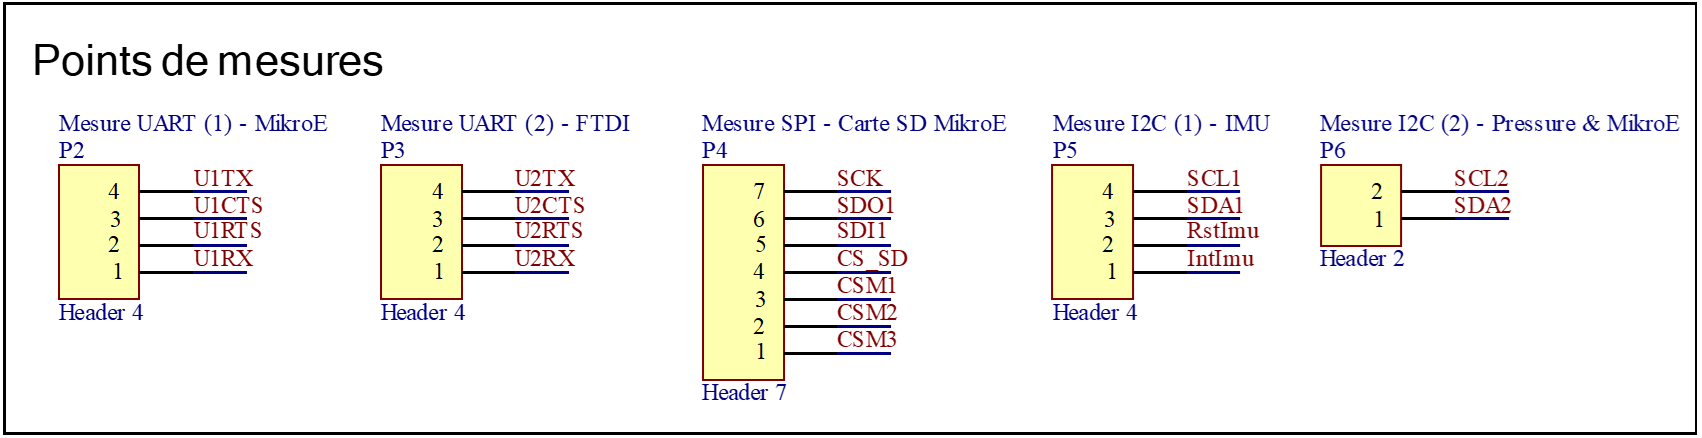
\includegraphics[width=0.9\linewidth]{Figures/Dev-SCH/PointsMesures}
			\caption{Connecteurs pour analyseur logique}
			\label{fig:pointsmesures}
		\end{figure}
		
		Une contrainte s'est crée, lorsque toutes les pins du microcontrôleur ont été allouée alors qu'il restait des connexion pour les "Chip select" et "Reset" des carte click-board Mikroe. Afin de remédier à ce problème, j'ai décidé d'utiliser un démultiplexeur, sachant que chacune des ces PINS, peuvent être activée seulement une à une : 
		
		\begin{figure}[h]
			\centering
			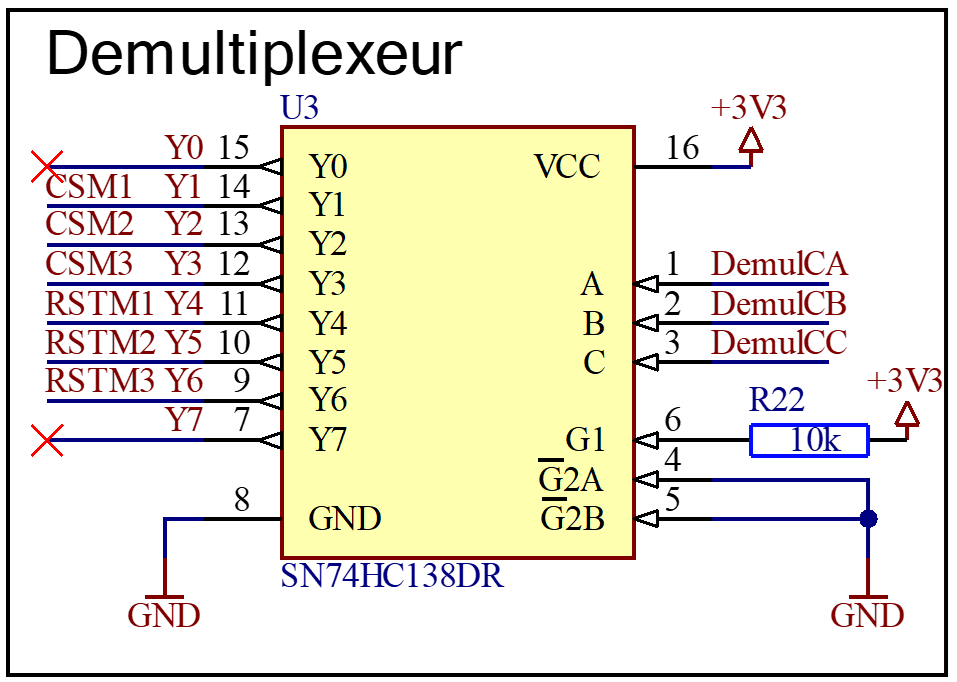
\includegraphics[width=0.6\linewidth]{Figures/Dev-SCH/Demultiplexeur}
			\caption{Demultiplexeur}
			\label{fig:demultiplexeur}
		\end{figure}
		

	}

	\clearpage
	\subsubsection{Chargeur de batterie} \label{sssec:BatCharger}
	{
		Ici je vais me pencher sur les dimensionnement des 3 résistances \textit{PROG} du composant de régulation et de charge d'accu, les autres composants passifs n'ont pas requis de dimensionnements particuliers.
		\begin{figure}[h]
			\centering
			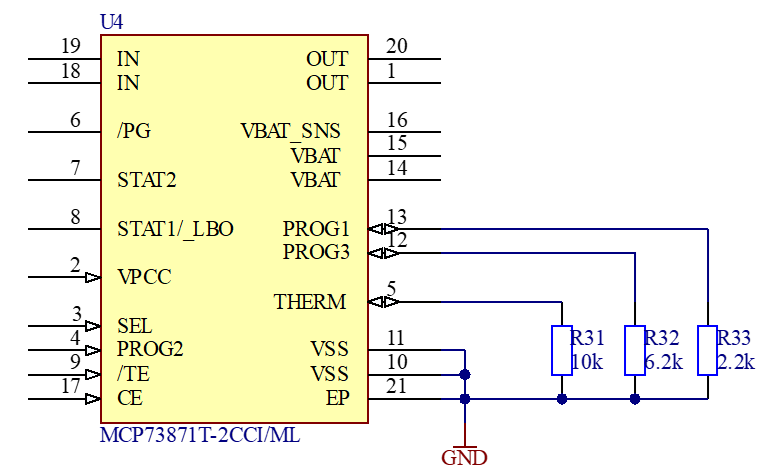
\includegraphics[width=0.55\linewidth]{Figures/Dev-SCH/ChargeBat}
			\caption{IC régulation et gestion charge de l'accu}
			\label{fig:chargebat}
		\end{figure}
		
		Afin de déterminer le comportement de la charge via les différentes étapes de courants, quelques équations ont été utiles : \\
		Où \\
		$C = 3400mAh$ \\
		$ratio_{term} = 0.05$
		$ratio_{chrg} = 0.1$
		
		\begin{equation} \label{equ:ich}
			I_{term} = C * ratio_{chrg} 
		\end{equation}
		D'après \ref{equ:ich}, $I_{term} = 170mA$.
	 
	 	\begin{equation} \label{equ:Rprog3}
		 	Rprog3 = \frac{1000V}{I_{term}}
		\end{equation}
		D'après \ref{equ:Rprog1}, $Rprog3 = 5k88 \Omega$ E12 $\Longrightarrow$ $6k2\Omega$ (Arrondis au supérieur pour limiter courant de terminaison).
		
		\begin{equation} \label{equ:Rprog1}
			Rprog1 = \frac{1000V}{C * ratio_{chrg}} 
		\end{equation}
		D'après \ref{equ:Rprog1}, $Rprog1 = 2k94 \Omega$ E12 $\Longrightarrow$ $2k2\Omega$ (Arrondis à l'inférieur pour limiter courant de charge).
		 
	}
	
	\clearpage
	\subsubsection{Conclusion et perspectives} \label{sssec:MethSchematic}
	{
		Lors du développement de la schématique, je n'ai pas eu de grands dimensionnements à faire mais plutôt dû mettre en place des mécanismes permettant la communication avec tous les senseurs et périphériques du système. J'ai essayé d'être le plus explicite possible lors de la création des différents blocs du schéma électrique, pour permettre une compréhension aisée de celui-ci. 
		
		J'ai pû faire un contrôle mutuel de la schématique avec mon collègue M. Meven Ricchieri.
		
		Je n'ai pas rencontré de problèmes particuliers, j'ai pus compléter la schématique, avancer sur le concept globale et je suis très enthousiaste de continuer ce projet.
		
		Désormais il vas falloir préparer la création du PCB, en contrôlant les footprints du circuit et développer d'avantage l'aspect mécanique du projet.
		
		La schématique issue de cette partie développement,  sera disponible en annexe de ce rapport.
		
		
	}
	

}


\clearpage